\section{Context}
\label{sec:context}

De gebruikers van het systeem zijn onder te verdelen in 5 categori\"{e}n: externen, studenten, professoren, assistenten en programmabeheerders. 
Elk soort gebruiker moet in de finale versie van CalZone in staat zijn de functionaliteiten die specifiek aan deze gebruikers zijn toegekend toe te passen zoals beschreven in het SRS\cite{SRS} van dit project. 
\\
In deze iteratie is de functionaliteit voor de administrator uitgebreid met de mogelijkheid om trajecten en vakken toe te voegen aan het systeem.
Ook werd functionaliteit opgestart om lessenroosters te gaan plannen.
\\

De functionaliteiten die iedere actor in het systeem bezit, worden ge\"{i}llustreerd in de use case diagrammen  \ref{fig:useCaseUsers}, \ref{fig:useCaseAdmin}, \ref{fig:useCaseProf} en \ref{fig:useCaseStudent}.

\begin{figure}[H]
	\centering
	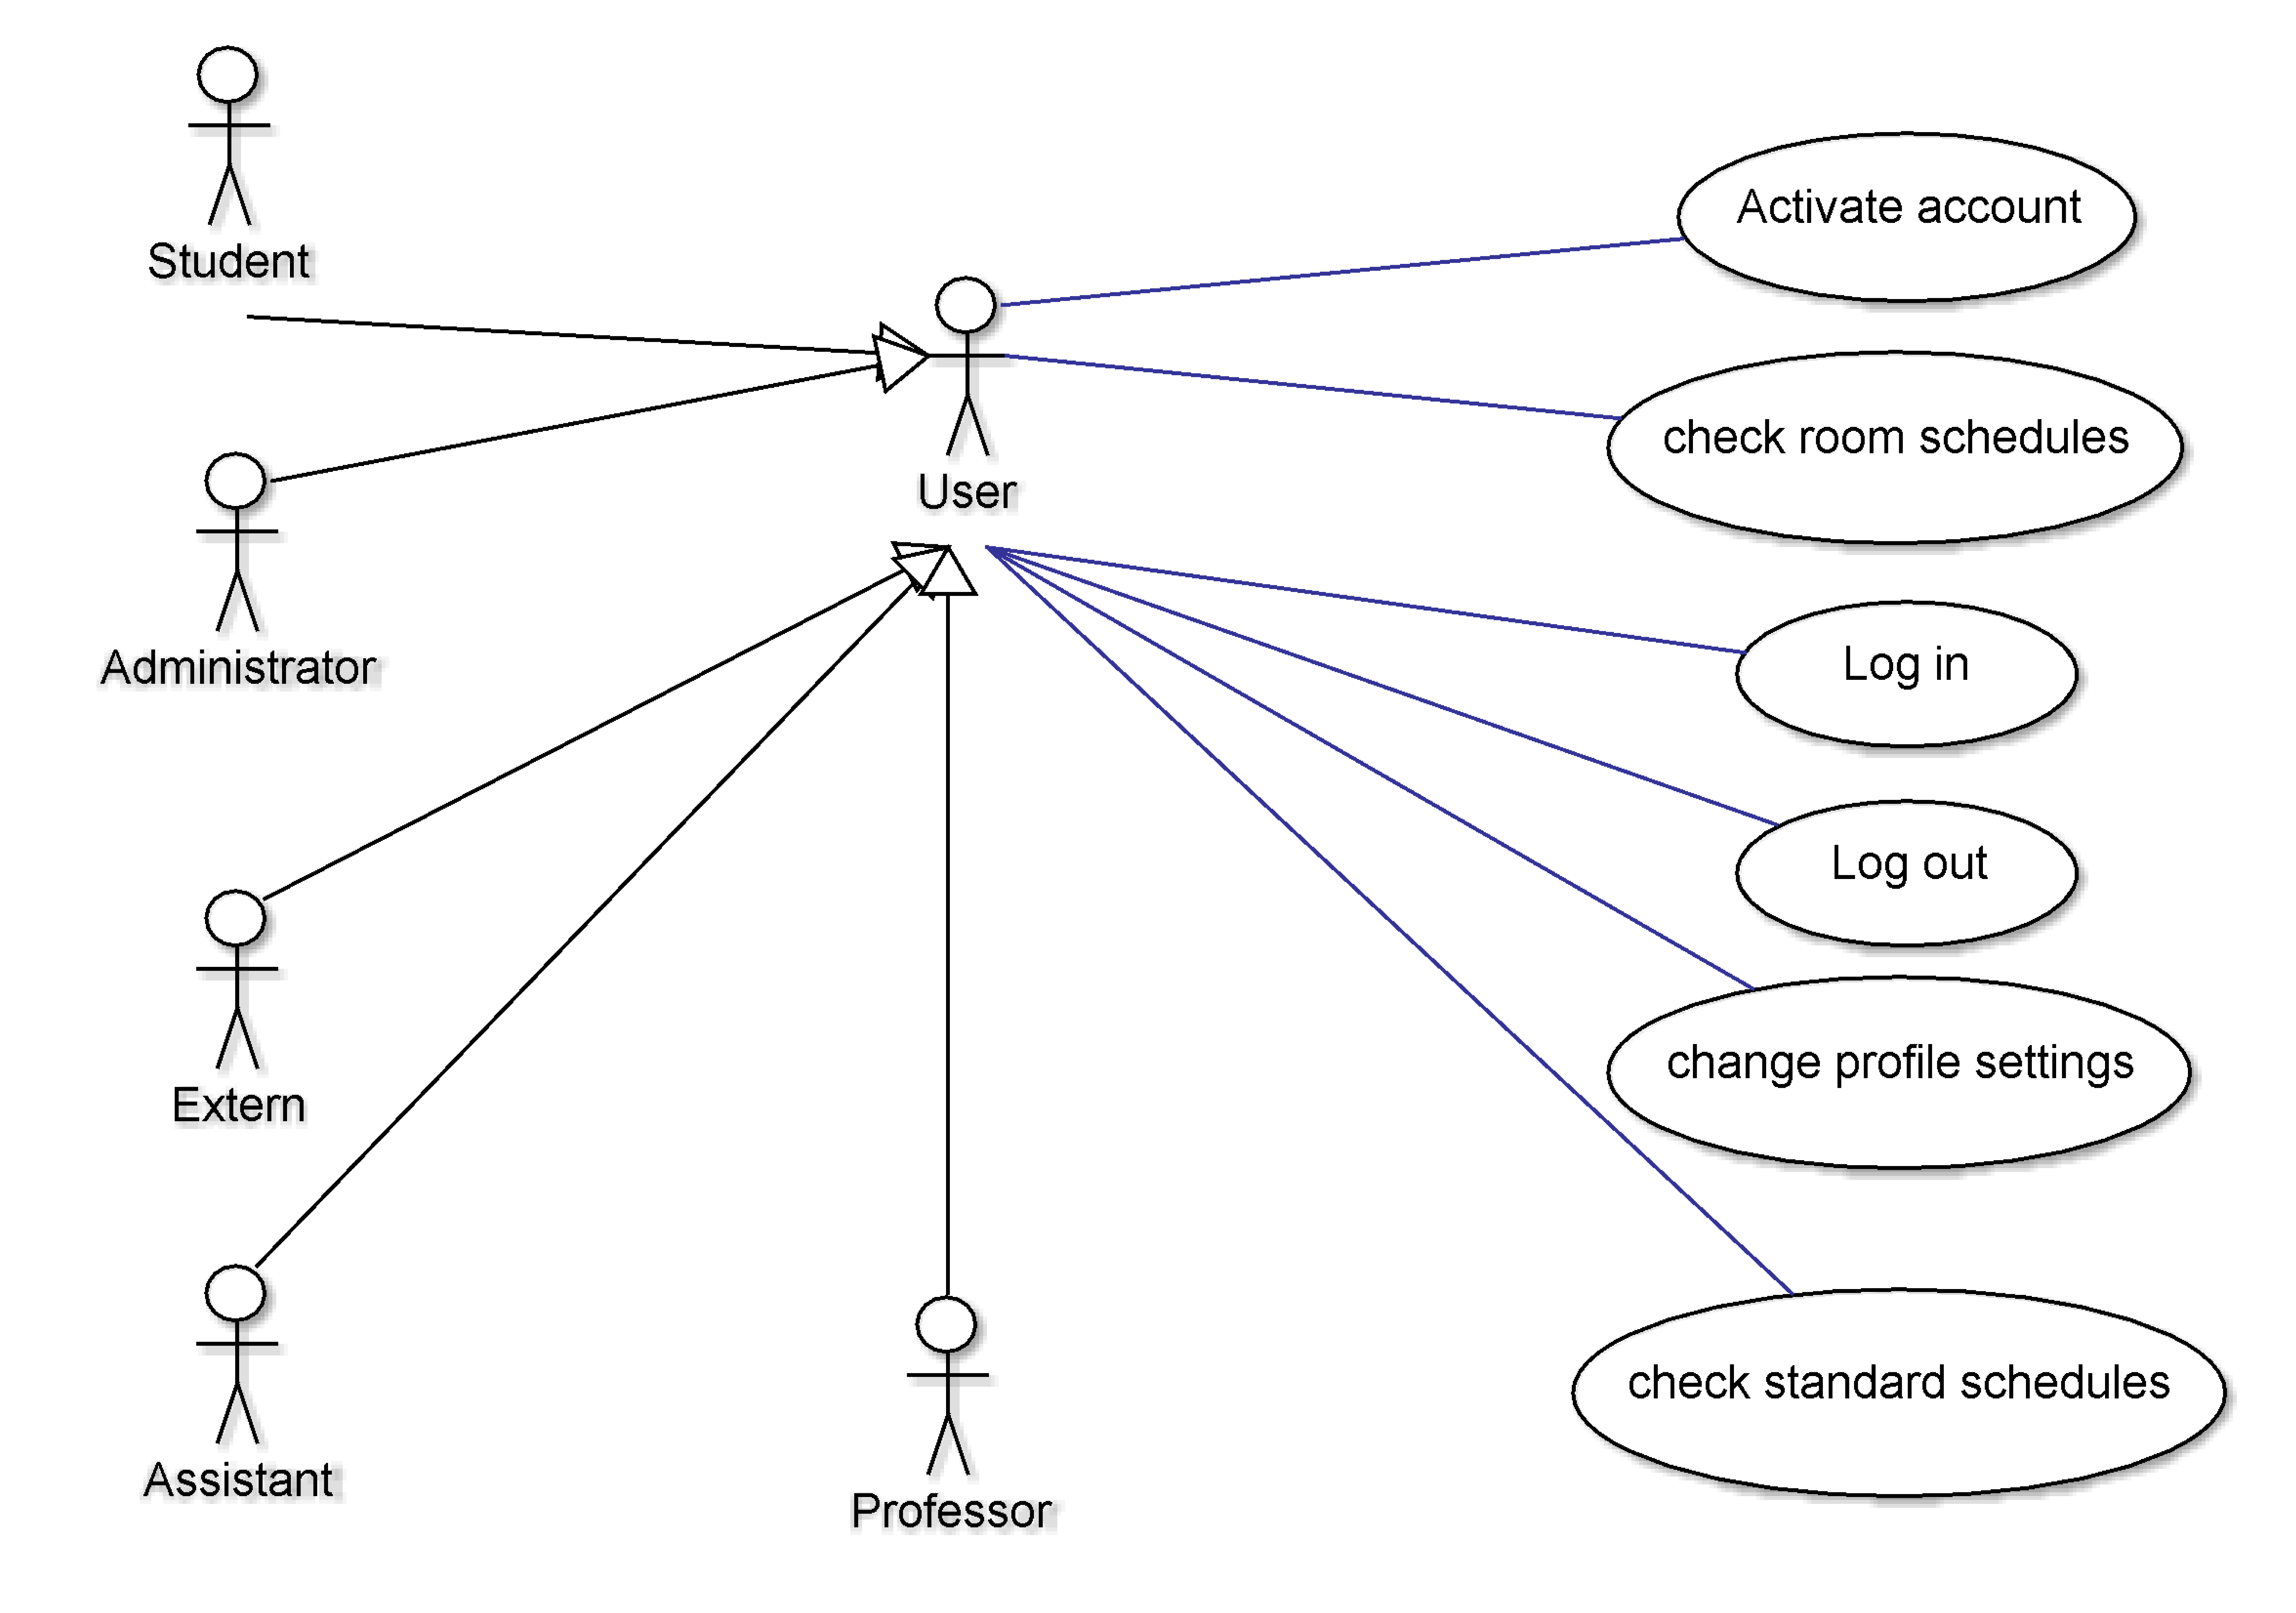
\includegraphics[scale=0.2]{img/useCaseUsers}
	\caption{Use case diagram met focus op de verschillende actoren}
	\label{fig:useCaseUsers}
\end{figure}

\begin{figure}[H]
	\centering
	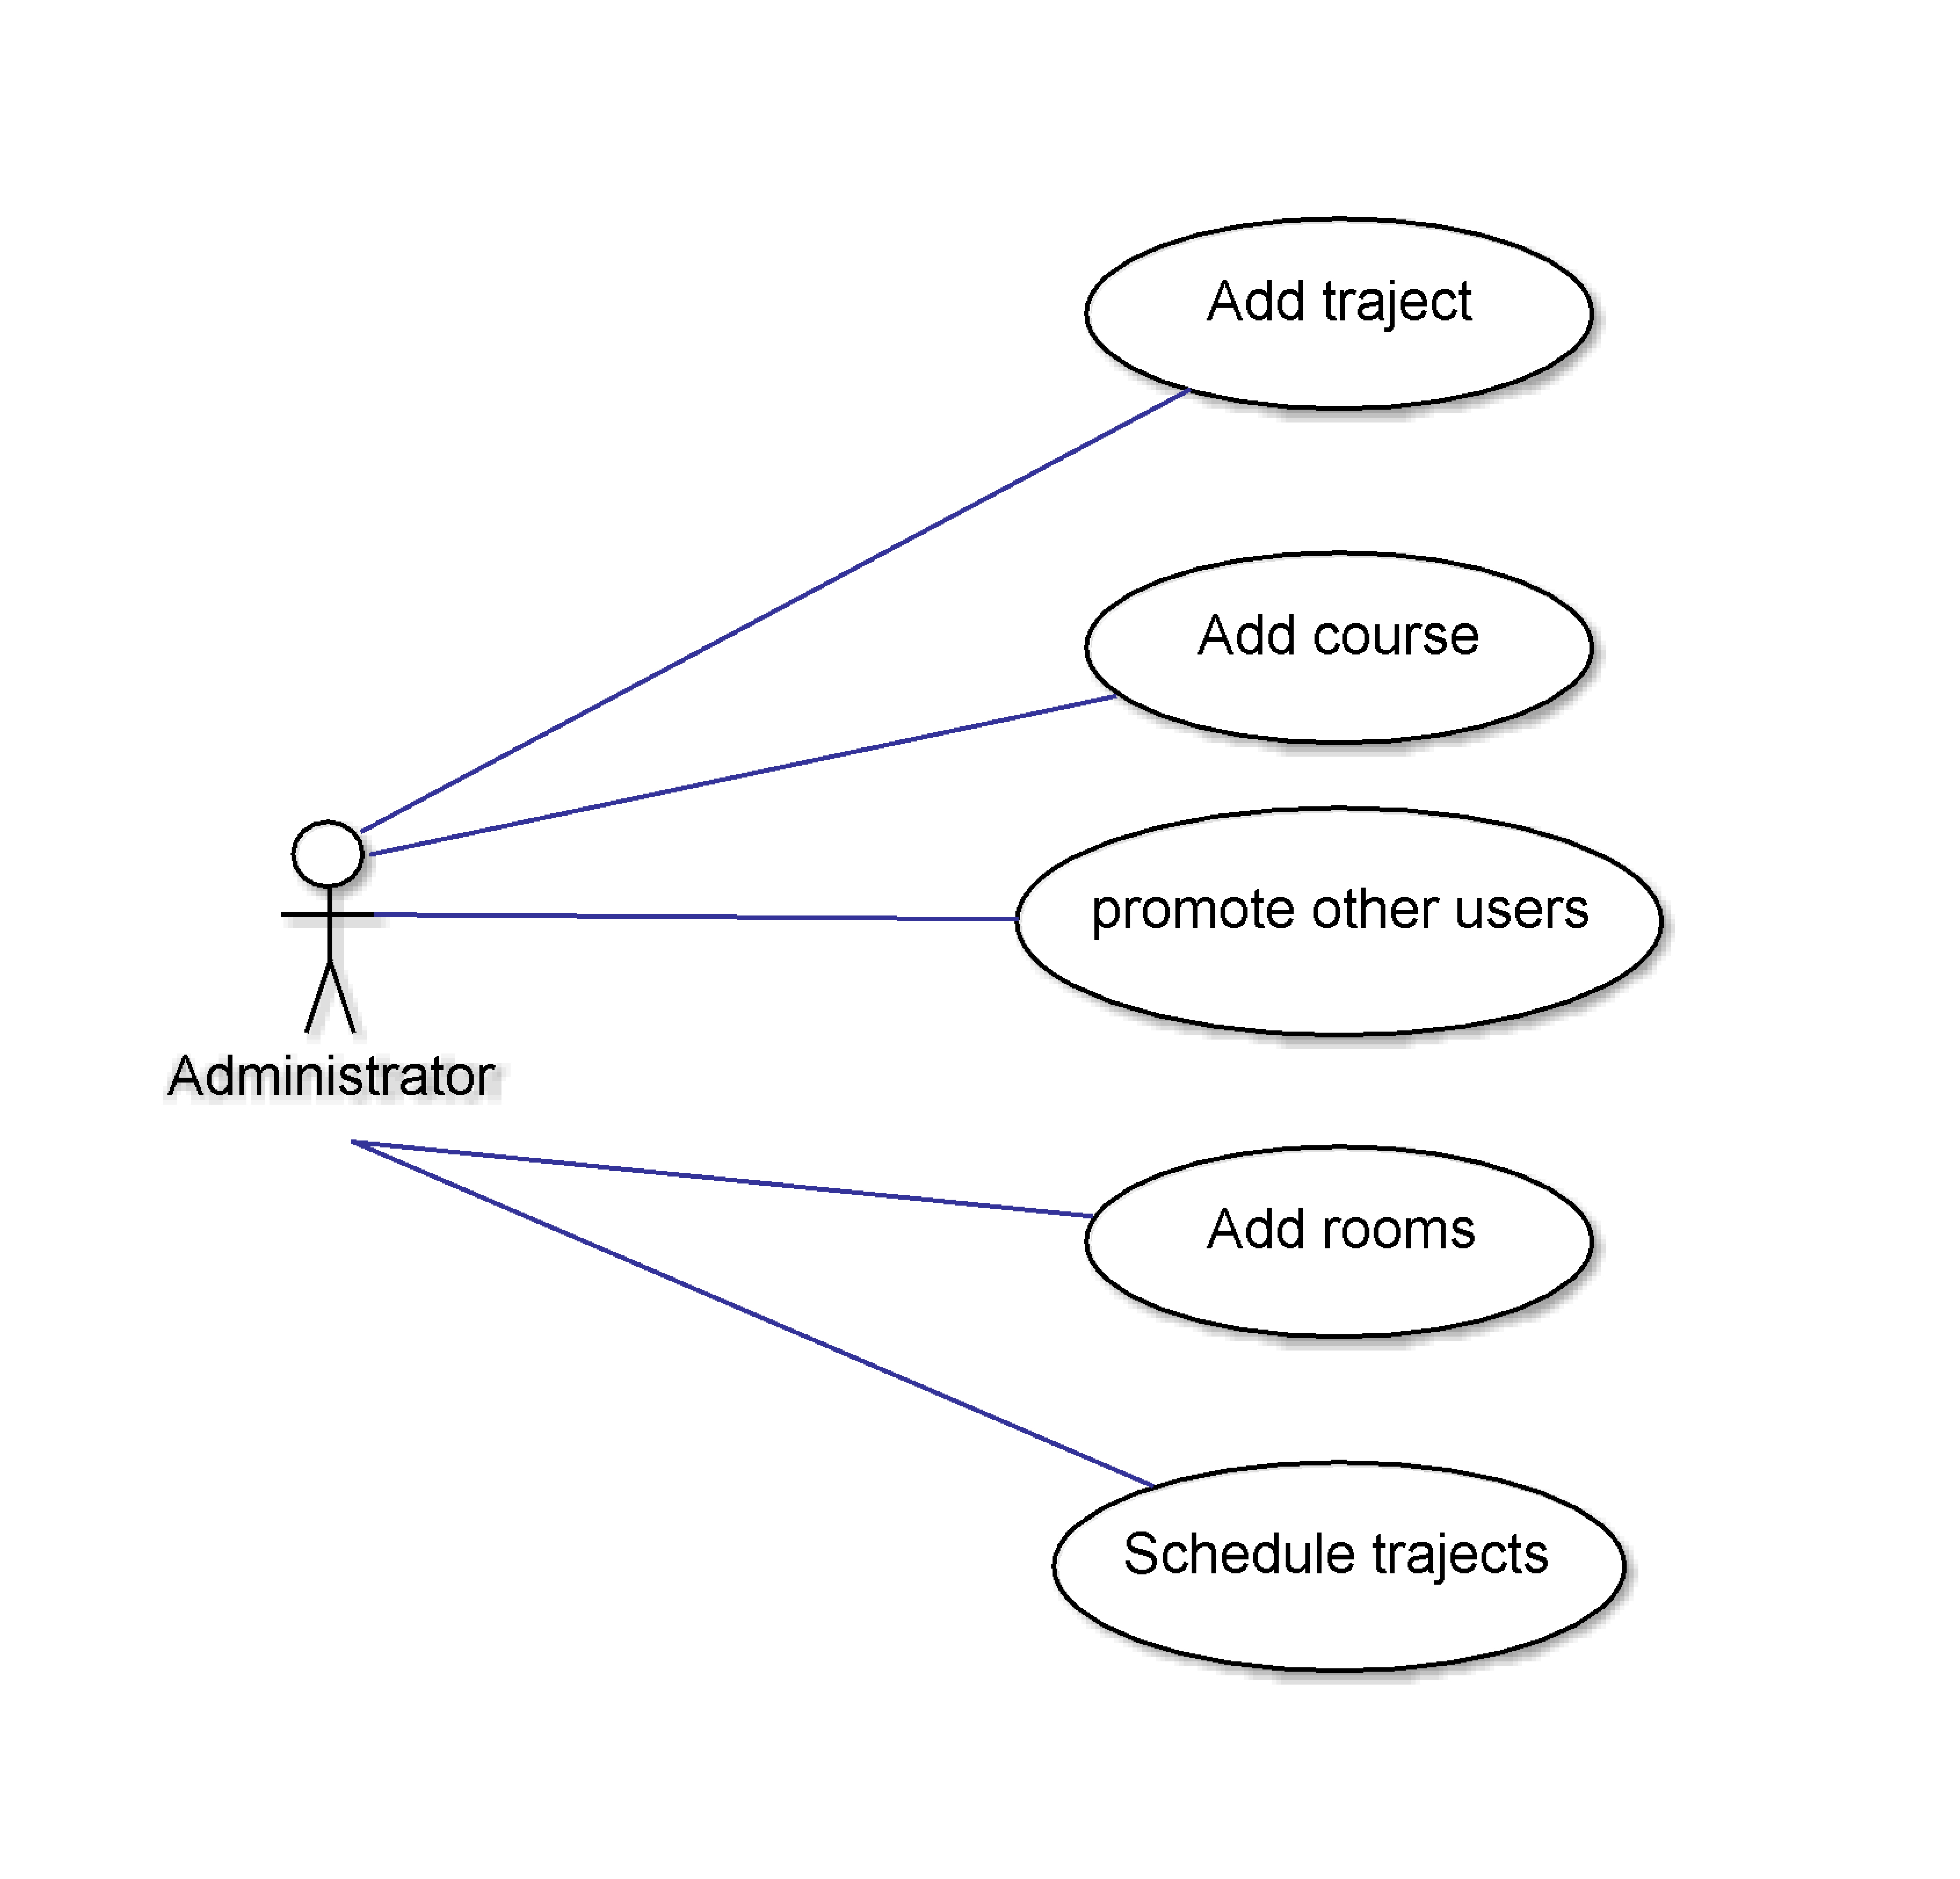
\includegraphics[scale=0.2]{img/useCaseAdmin}
	\caption{Use case diagram met focus op de actor Administrator}
	\label{fig:useCaseAdmin}
\end{figure}

\begin{figure}[H]
	\centering
	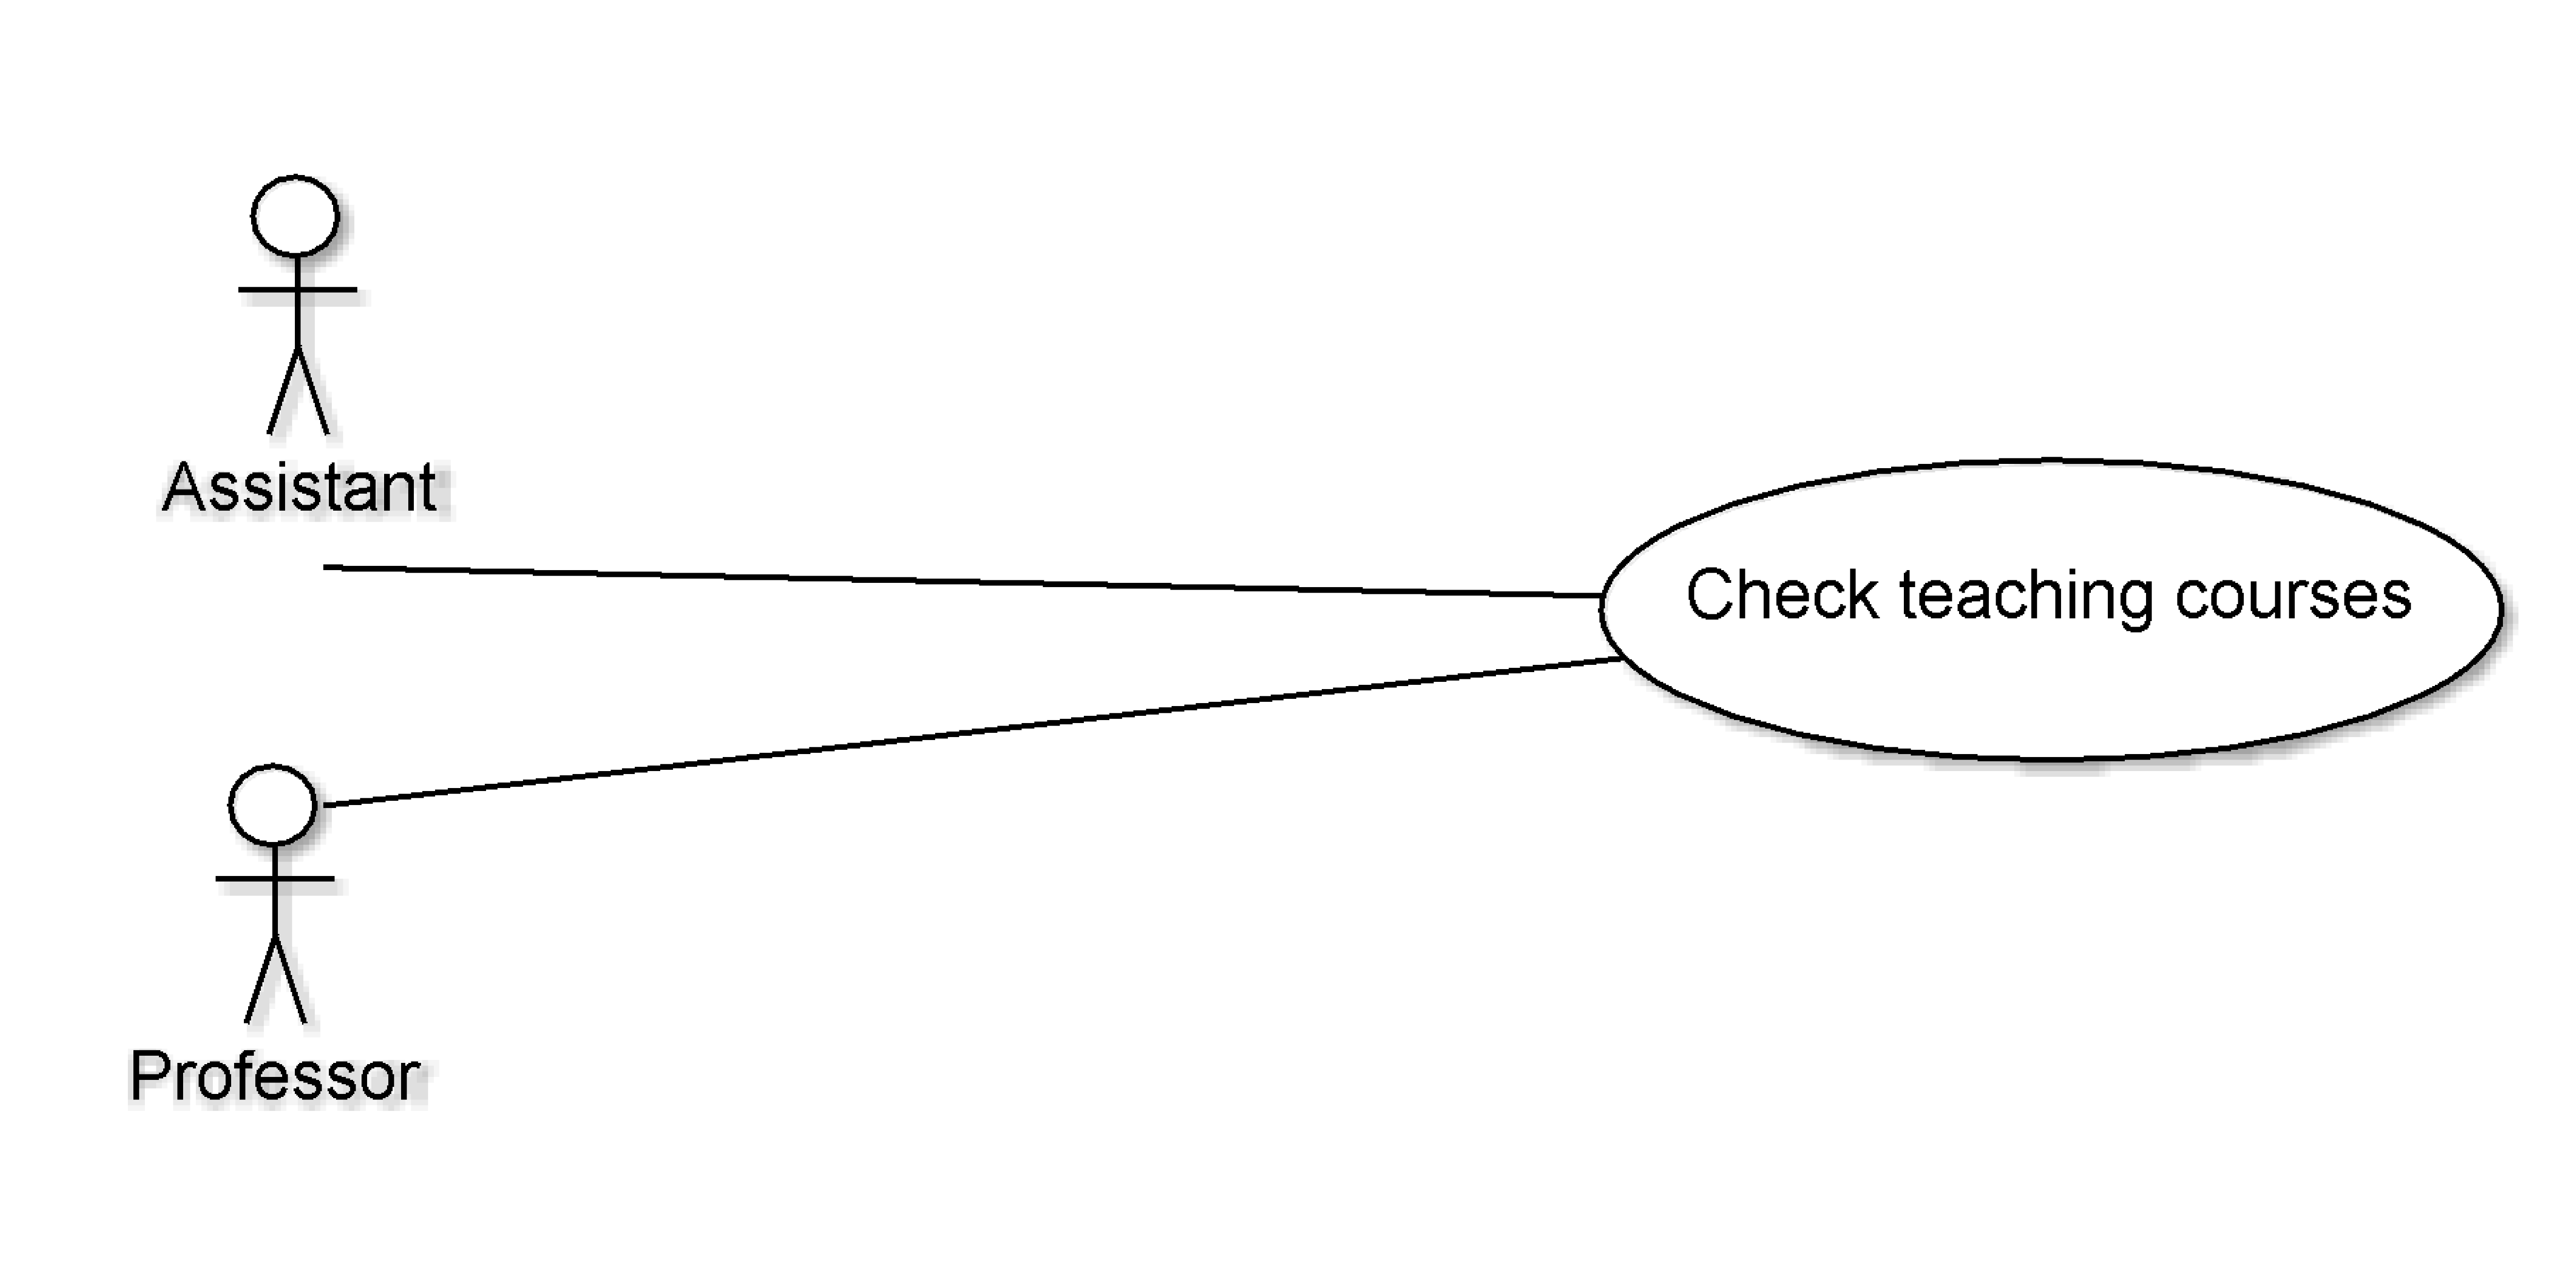
\includegraphics[scale=0.2]{img/useCaseProf}
	\caption{Use case diagram met focus op de actoren Professor en Assistant}
	\label{fig:useCaseProf}
\end{figure}

\begin{figure}[H]
	\centering
	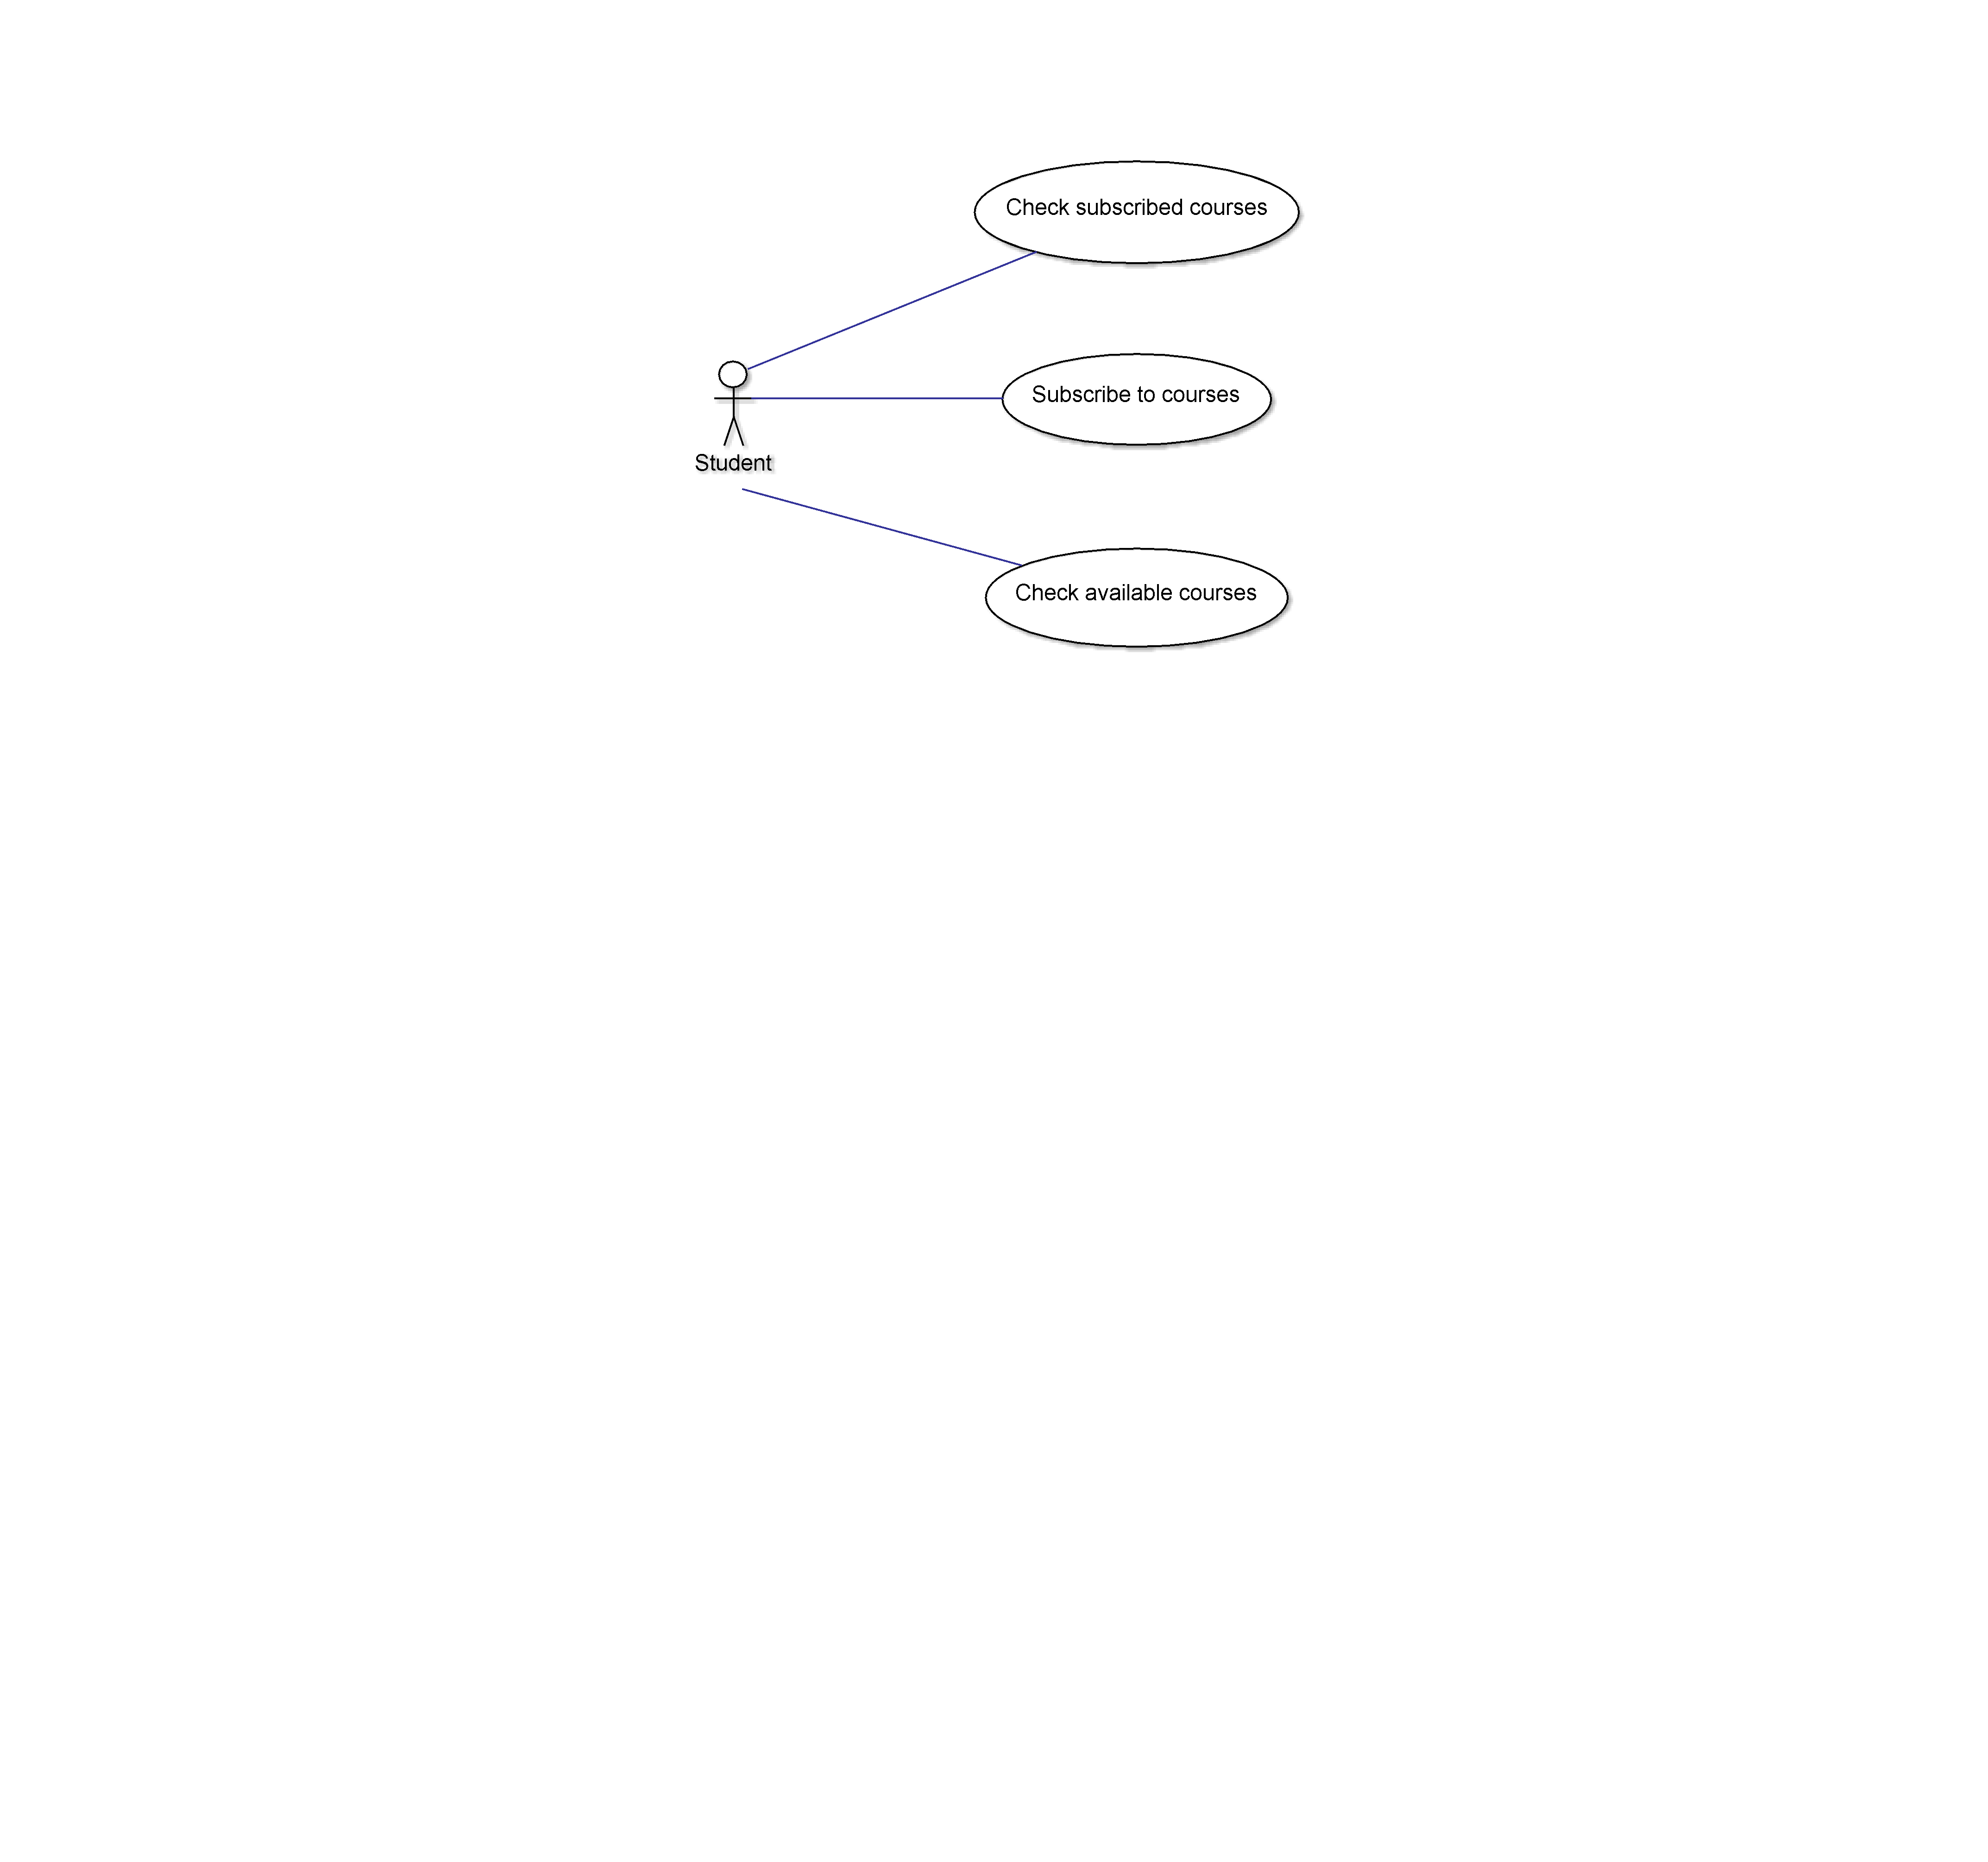
\includegraphics[scale=0.2]{img/useCaseStudent}
	\caption{Use case diagram met focus op de actor Student}
	\label{fig:useCaseStudent}
\end{figure}